\documentclass{article}

\usepackage{graphicx}
\usepackage{tikz}
\usepackage{tikzsymbols}
\usetikzlibrary{calc,patterns,shapes.geometric}
\pagestyle{empty}
\usepackage[margin=0pt]{geometry}
\geometry{papersize={14in,12in}}

\def\centerarc[#1](#2)(#3:#4:#5){\draw[#1] ($(#2)+({#5*cos(#3)},{#5*sin(#3)})$) arc (#3:#4:#5);}

\begin{document}
	\begin{figure}
		\centering
		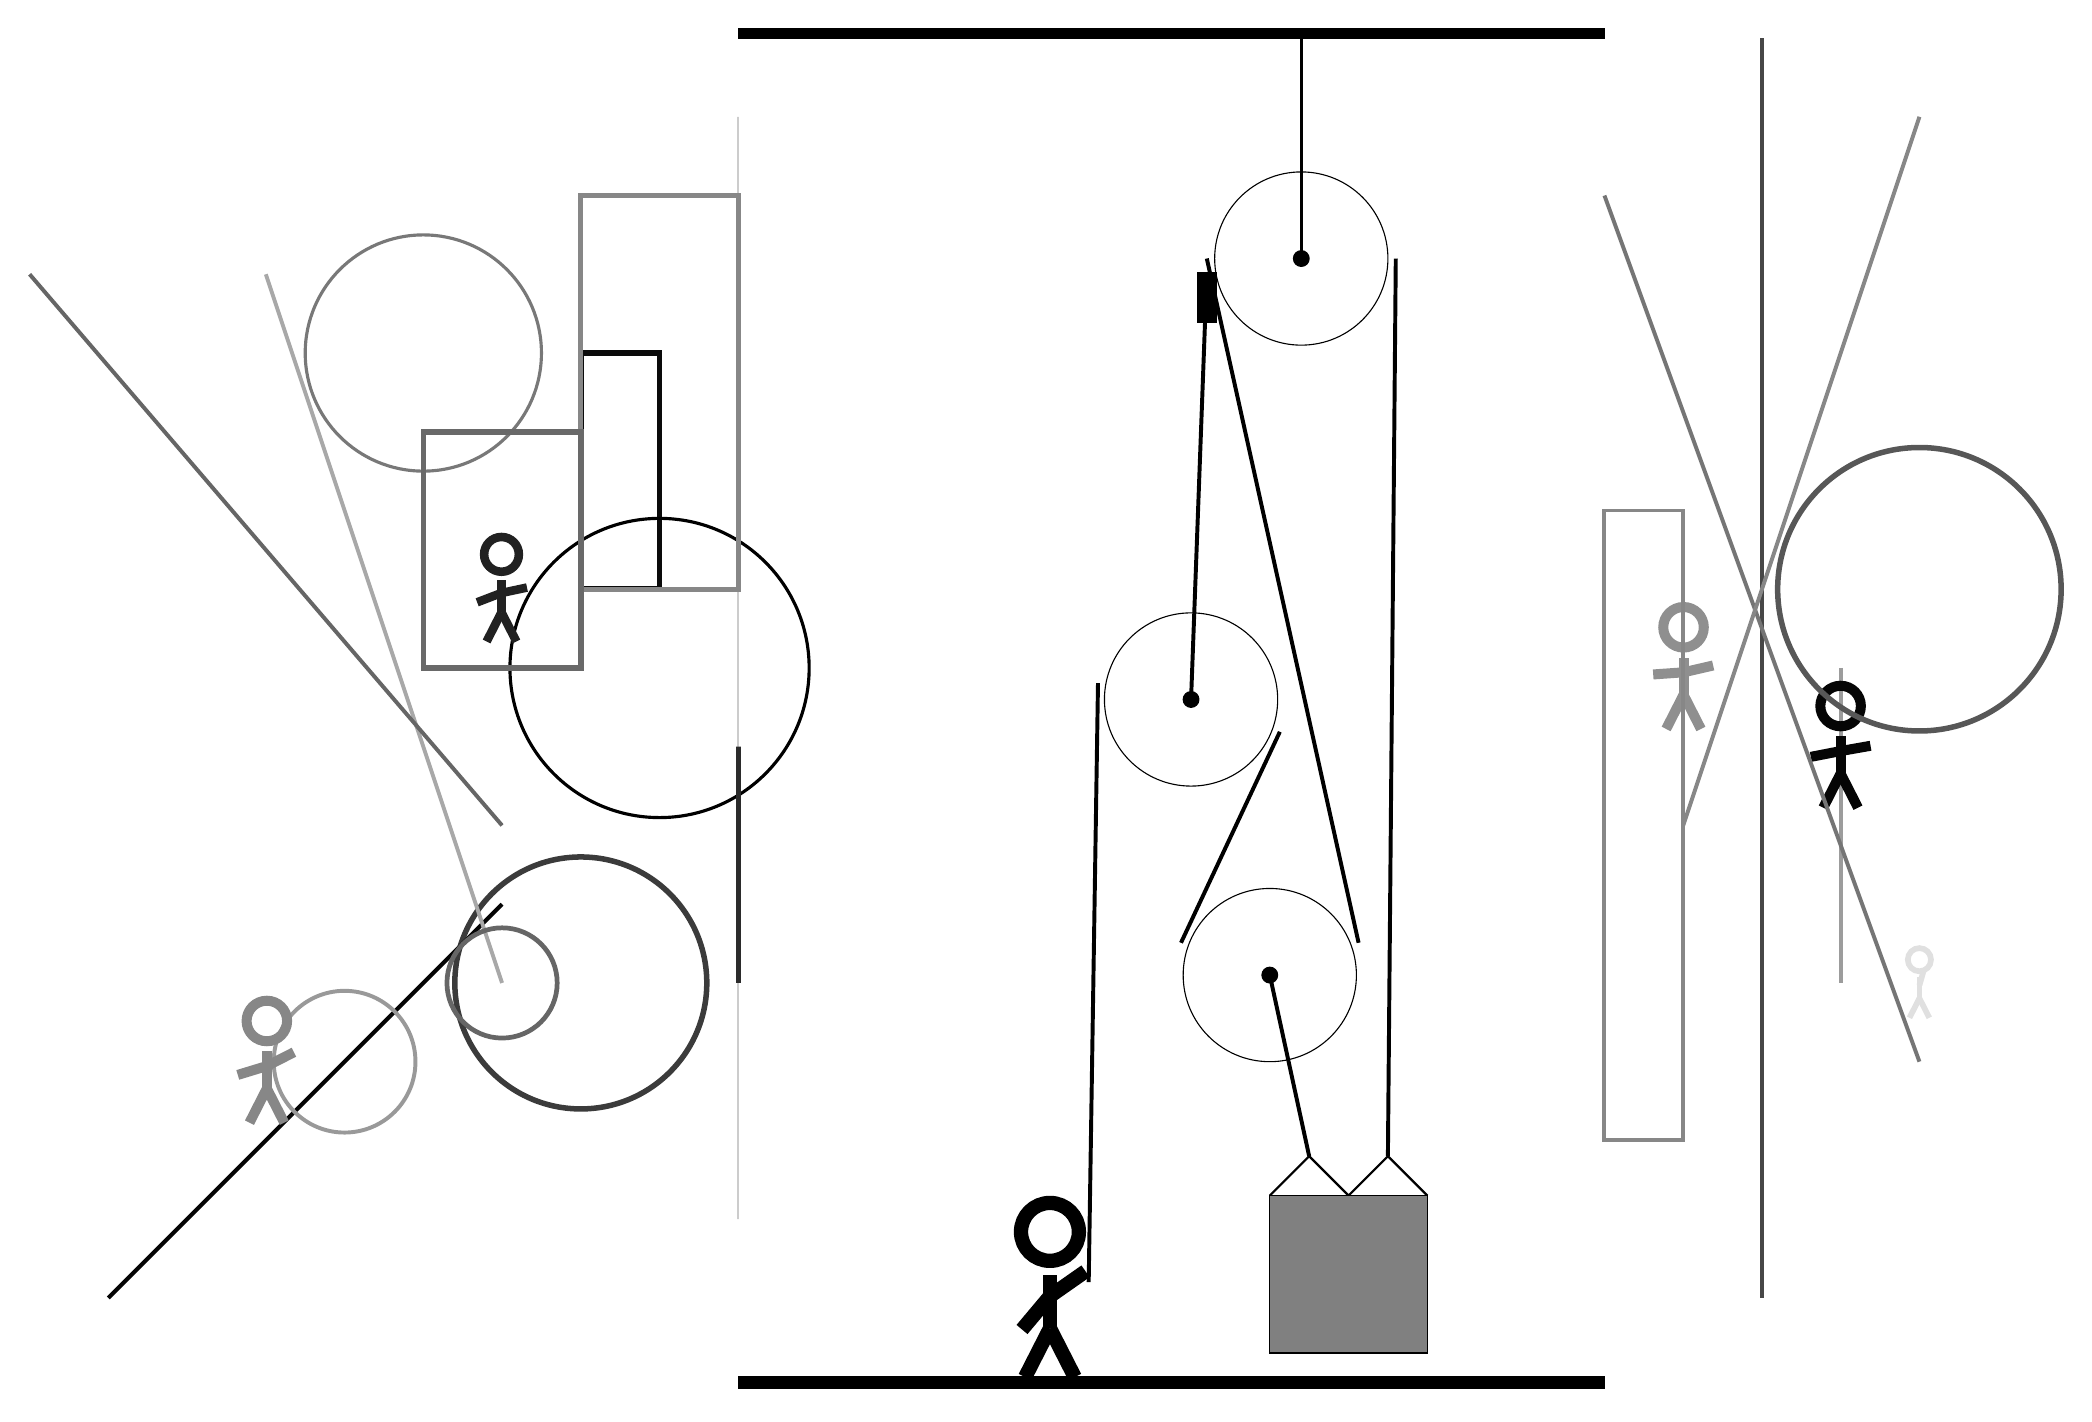
\begin{tikzpicture}
			%%%%% START %%%%%
			
			\draw[fill=black] (-6, 14) rectangle (5, 14.125);
			
			\draw (-0.25, 5.6) circle (1.1);
			\draw[fill=black] (-0.25, 5.6) circle (0.1);
			
			\draw (0.75, 2.1) circle (1.1);
			\draw[fill=black] (0.75, 2.1) circle (0.1);
			
			\draw (1.15, 11.2) circle (1.1);
			\draw[fill=black] (1.15, 11.2) circle (0.1);
			\draw[very thick] (1.15, 11.2) -- (1.15, 14);
			
			\draw[thick]  (0.75, -0.7) -- (1.25, -0.2) -- (1.75, -0.7) -- (2.25, -0.2) -- (2.75, -0.7);
			\draw[fill=black!50] (0.75, -0.7) rectangle (2.75, -2.7);
			
			\draw[line width=0.5mm] (-0.25, 5.6) -- (-0.05, 11.0);
			\draw[line width=0.5mm, fill=black](-0.15, 10.4) rectangle (0.05, 11.0);
			\draw[line width=0.5mm] (-1.55, -1.8) -- (-1.4318, 5.8083);
			\centerarc[line width=0.5mm](-0.25, 5.6)(-20:170:1.2000000000000002);
			\draw[line width=0.5mm] (0.8776, 5.1896) -- (-0.3776, 2.5104);
			\centerarc[line width=0.5mm](0.75, 2.1)(160:380:1.2000000000000002);
			\draw[line width=0.5mm] (1.8776, 2.5104) -- (-0.05, 11.2);
			\draw[line width=0.5mm](0.75, 2.1) -- (1.25, -0.2);
			\centerarc[line width=0.5mm](1.15, 11.2)(0:180:1.2000000000000002);
			\draw[line width=0.5mm] (2.35, 11.2) -- (2.25, -0.2);
			
			\draw[line width=0.6mm, color=black!72] (7, -2) rectangle (7, 14);
			
			\draw[line width=0.7mm, color=black!96] (-8, 7) rectangle (-7, 10);
			\draw [line width=0.4mm, color=black!100](-7, 6) circle (1.9);
			\draw[line width=0.5mm, color=black!39](8, 6) -- (8, 2);
			\draw [line width=0.4mm, color=black!53](-10, 10) circle (1.5);
			
			\node[line width=0.2mm, color=black!98] at (8, 5) {\Strichmaxerl[7][11][10]};
			\draw [line width=0.7mm, color=black!77](-8, 2) circle (1.6);
			\draw [line width=0.7mm, color=black!66](9, 7) circle (1.8);
			\draw[line width=0.3mm, color=black!20] (-6, -1) rectangle (-6, 13);
			\node[line width=0.3mm, color=black!87] at (-9, 7) {\Strichmaxerl[6][21][12]};
			\draw[line width=0.5mm, color=black!98](-9, 3) -- (-14, -2);
			
			\draw[line width=0.5mm, color=black!54](5, 12) -- (9, 1);
			\draw [line width=0.5mm, color=black!40](-11, 1) circle (0.9);
			\draw[line width=0.5mm, color=black!34](-9, 2) -- (-12, 11);
			\draw [line width=0.6mm, color=black!60](-9, 2) circle (0.7);
			\node[line width=0.5mm, color=black!44] at (6, 6) {\Strichmaxerl[7][4][13]};
			
			\draw[line width=0.6mm, color=black!47] (-8, 12) rectangle (-6, 7);
			\draw[line width=0.7mm, color=black!59] (-8, 6) rectangle (-10, 9);
			\draw[line width=0.5mm, color=black!47] (5, 8) rectangle (6, 0);
			\draw[line width=0.5mm, color=black!47](9, 13) -- (6, 4);
			\node[line width=0.2mm, color=black!12] at (9, 2) {\Strichmaxerl[4][90][74]};
			
			\node[line width=0.5mm, color=black!47] at (-12, 1) {\Strichmaxerl[7][17][27]};
			\draw[line width=0.5mm, color=black!60](-9, 4) -- (-15, 11);
			\draw[line width=0.6mm, color=black!83] (-6, 5) rectangle (-6, 2);
			
			\node at (-2, -1.9) {\Strichmaxerl[10][50][35]};
			
			\draw[fill=black] (-6, -3) rectangle (5, -3.15);
			
			%%%%% END %%%%%
		\end{tikzpicture}
	\end{figure}	
\end{document}